\section{Full adder as network}\label{app:Full_adder}
To create a full adder from basic neurons, the corresponding logic gates need to be defined. The equivalent neuron for an ''and''-gate was defined in \autoref{sec:basics_neuron_network}. There are two more basic neurons which will be defined here. The neuron corresponding to the ''or''-gate, which is given by the same activation function \eqref{def:step_activation}, weights $\vec{w}={(w_1, w_2)}^T=(1,1)$ and bias $b=-0.5$, and the neuron equivalent to the ''not''-gate, which is given by the activation function \eqref{def:step_activation}, weight $w=-1$ and bias $b=0.5$. These definitions are summarized in \autoref{tab:neuron_logic_gates}.
\begin{table}[H]
\begin{center}
\begin{tabular}{c|c|c}
''and''-neuron & ''or''-neuron & ''not''-neuron\\
\hline
\begin{tikzpicture}[
neuron/.style={circle, draw=black, very thick, minimum size=1.0cm},
dot/.style={circle, draw=black, fill=black, minimum size=0.1cm, inner sep=0pt},
VLineVertex/.style={circle, draw=black, minimum size=0cm, inner sep=0pt},
]

\node[neuron] (neuron) {\textbf{and}};
\node (place) [left=1cm of neuron] {};
\node (x1) [above=0.25cm of place] {$x_1$};
\node (x3) [below=0.25cm of place] {$x_3$};
\node (out) [right=0.75cm of neuron] {$x_1\land x_2$};

\draw (x1.east) -- (neuron.west);
\draw (x3.east) -- (neuron.west);
\draw [->] (neuron.east) -- (out.west);

\end{tikzpicture} & \begin{tikzpicture}[
neuron/.style={circle, draw=black, very thick, minimum size=1.0cm},
dot/.style={circle, draw=black, fill=black, minimum size=0.1cm, inner sep=0pt},
VLineVertex/.style={circle, draw=black, minimum size=0cm, inner sep=0pt},
]

\node[neuron] (neuron) {\textbf{or}};
\node (place) [left=1cm of neuron] {};
\node (x1) [above=0.25cm of place] {$x_1$};
\node (x3) [below=0.25cm of place] {$x_3$};
\node (out) [right=0.75cm of neuron] {$x_1\lor x_2$};

\draw (x1.east) -- (neuron.west);
\draw (x3.east) -- (neuron.west);
\draw [->] (neuron.east) -- (out.west);

\end{tikzpicture} & \begin{tikzpicture}[
neuron/.style={circle, draw=black, very thick, minimum size=1.0cm},
dot/.style={circle, draw=black, fill=black, minimum size=0.1cm, inner sep=0pt},
VLineVertex/.style={circle, draw=black, minimum size=0cm, inner sep=0pt},
]

\node[neuron] (neuron) {\textbf{not}};
\node (x1) [left=0.65cm of neuron] {$x_1$};
\node (out) [right=0.65cm of neuron] {$\lnot x_1$};

\draw (x1.east) -- (neuron.west);
\draw [->] (neuron.east) -- (out.west);

\end{tikzpicture}\\
\hline
\begin{tabular}{c c}
$\vec{w}=(1,1)$ & $b=-1.5$
\end{tabular} &
\begin{tabular}{c c}
$\vec{w}=(1,1)$ & $b=-0.5$
\end{tabular} &
\begin{tabular}{c c}
$w=-1$ & $b=0.5$
\end{tabular}\\
\hline
\begin{tabular}{c c|c}
$x_1$ & $x_2$ & $a(x_1+x_2-1.5)$\\
\hline
$0$ & $0$ & $0$\\
$0$ & $1$ & $0$\\
$1$ & $0$ & $0$\\
$1$ & $1$ & $1$\\
\end{tabular} &
\begin{tabular}{c c|c}
$x_1$ & $x_2$ & $a(x_1+x_2-0.5)$\\
\hline
$0$ & $0$ & $0$\\
$0$ & $1$ & $1$\\
$1$ & $0$ & $1$\\
$1$ & $1$ & $1$\\
\end{tabular} &
\begin{tabular}{c|c}
$x_1$ & $a(-x_1+0.5)$\\
\hline
$0$ & $1$\\
$1$ & $0$\\
\end{tabular}
\end{tabular}
\end{center}
\caption[Logic gates as neurons]{A summary and depiction of the main logic gates written as neurons. All of them share the same activation function \eqref{def:step_activation}.}\label{tab:neuron_logic_gates}
\end{table}
\medskip
\noindent Using the basic logic gates a more complex structure - the ''XOR''-gate - can be built. A ''XOR''-gate is defined by its truth table (see \autoref{tab:xor}).
\begin{table}[H]
\centering
\begin{tabular}{c c|c}
$x_1$ & $x_2$ & $x_1\veebar x_2$\\
\hline
$0$ & $0$ & $0$\\
$0$ & $1$ & $1$\\
$1$ & $0$ & $1$\\
$1$ & $1$ & $0$
\end{tabular}
\caption[Truth table for  the ''XOR''-gate]{Truth table for the ''XOR''-gate.}\label{tab:xor}
\end{table}
It can be constructed from the three basic logic operations ''and'', ''or'' and ''not''
\begin{equation}
x_1\veebar x_2 = \lnot\lr{\lr{x_1\land x_2}\lor\lnot\lr{x_1\lor x_2}}.
\end{equation}
Therefore the basic neurons from \autoref{tab:neuron_logic_gates} can be combined to create a ''XOR''-network (see \autoref{fig:xor_net}).\\
To simplify readability from here on out a neuron called ''XOR'' will be used. It is defined by the network of \autoref{fig:xor_net} and has to be replaced by it, whenever it is used.\\
With this ''XOR''-neuron a network, that behaves like a full-adder, can be defined. A full-adder is a binary adder with carry in and carry out, as seen in \autoref{fig:full_adder}.
\begin{figure}[H]
\centering
\begin{tikzpicture}[
neuron/.style={circle, draw=black, very thick, minimum size=1.0cm},
dot/.style={circle, draw=black, fill=black, minimum size=0.1cm, inner sep=0pt},
VLineVertex/.style={circle, draw=black, minimum size=0cm, inner sep=0pt},
]

\node[neuron] (out_not) {\textbf{not}};
\node[neuron] (final_or) [left=1cm of out_not] {\textbf{or}};
\node (between) [left=1cm of final_or] {};
\node[neuron] (bot_not) [below=0.25cm of between] {\textbf{not}};
\node[neuron] (bot_or) [left=1cm of bot_not] {\textbf{or}};
\node[neuron] (x2) [left=1cm of bot_or] {$x_2$};
\node[neuron] (x1) [above=0.5cm of x2] {$x_1$};
\node[neuron] (top_and) [right=2cm of x1] {\textbf{and}};
\node (out) [right=0.5cm of out_not] {$x_1\veebar x_2$};

%Input
\draw (x1.east) -- (top_and.west);
\draw (x2.east) -- (top_and.west);
\draw (x1.east) -- (bot_or.west);
\draw (x2.east) -- (bot_or.west);

%First and second layer connections
\draw (top_and.east) -- (final_or.west);
\draw (bot_or.east) -- (bot_not.west);
\draw (bot_not.east) -- (final_or.west);

%Final connection
\draw (final_or.east) -- (out_not.west);

%Output
\draw [->] (out_not.east) -- (out.west);
\end{tikzpicture}
\caption[''XOR''-network]{The definition of a network that is equivalent to an ''XOR''-gate.}\label{fig:xor_net}
\end{figure}
\begin{figure}[H]
\centering
\begin{tikzpicture}[
neuron/.style={circle, draw=black, very thick, minimum size=1.4cm},
dot/.style={circle, draw=black, fill=black, minimum size=0.1cm, inner sep=0pt},
VLineVertex/.style={circle, draw=black, minimum size=0cm, inner sep=0pt},
]

\node[neuron] (x1) {$x_1$};
\node[neuron] (x2) [below=0.5cm of x1] {$x_2$};
\node[neuron] (x3) [below=0.5cm of x2] {$x_3$};
\node (center_xor1) [below=0.25cm of x1] {};
\node[neuron] (xor1) [right=1.5cm of center_xor1] {\textbf{XOR}};
\node[neuron] (xor2) [right=4.1cm of x2] {\textbf{XOR}};
\node[neuron] (and1) [below=0.5cm of xor2] {\textbf{and}};
\node[neuron] (and2) [below=0.5cm of and1] {\textbf{and}};
\node (center_or1) [below=0.25cm of and1] {};
\node[neuron] (or1) [right=1cm of center_or1] {\textbf{or}};
\node (out_sum) [right=2.5cm of xor2] {Sum};
\node (out_car) [right=0.5cm of or1] {$\text{Carry}_\text{out}$};

%Inputs
\node (x1_in) [left=0.5cm of x1] {$x_1$};
\node (x2_in) [left=0.5cm of x2] {$x_2$};
\node (car_in) [left=0.5cm of x3] {$\text{Carry}_\text{in}$};

%Draw lines
%Input arrows
\draw[->] (x1_in.east) -- (x1.west);
\draw[->] (x2_in.east) -- (x2.west);
\draw[->] (car_in.east) -- (x3.west);

%Input connections
\draw (x1.east) -- (xor1.west);
\draw (x1.east) -- (and2.west);
\draw (x2.east) -- (xor1.west);
\draw (x2.east) -- (and2.west);
\draw (x3.east) -- (xor2.west);
\draw (x3.east) -- (and1.west);

%xor1 connections
\draw (xor1.east) -- (xor2.west);
\draw (xor1.east) -- (and1.west);

%Third layer connections
\draw[->] (xor2.east) -- (out_sum.west);
\draw (and1.east) -- (or1.west);
\draw (and2.east) -- (or1.west);

%Or out
\draw[->] (or1.east) -- (out_car.west);
\end{tikzpicture}
\caption[Full adder network]{A network replicating the behavior of a binary full adder.}\label{fig:full_adder}
\end{figure}

\section{Indication that the network does not learn}\label{app:network_does_not_learn}
Sometimes during training only a local minimum is found. The most notable of these minima is when the network just picks a fixed value in the interval and appoints it to any input. It is therefore useful to spot this behavior during training and consider restarting. Therefore the value for a constant output will be calculated in this appendix.
\medskip\\
To start off the loss function will be assumed to be the mean squared error. Furthermore it is assumed, that the \gls{snr}-values lie within the interval $\left[a,b\right]$. The mean squared error of a chosen point $x$ to every point in this interval is given by
\begin{equation}
f(x)\coloneqq\frac{1}{b-a}\int_a^b\diff y\ \lr{x-y}^2=\frac{1}{3\lr{b-a}}\lr{\lr{b-x}^3-\lr{a-x}^3}.
\end{equation}
To minimize this one could in principle solve $\frac{\partial f}{\partial x}\mbe 0$ and it would yield the correct result. However it should at least intuitively be obvious that the point that minimizes the mean squared error to every point in the interval is the mean value of the interval $x=\frac{a+b}{2}$.\\
Therefore if the network has to choose values out of a given interval $\left[a,b\right]$, minimize the mean squared error and the training finds a local minimum that leads to the network always returning a fixed value, this value should be
\begin{equation}
f\lr{\frac{a+b}{2}}=\frac{1}{3\lr{b-a}}\lr{\lr{\frac{b-a}{2}}^3-\lr{\frac{a-b}{2}}^3}=\frac{1}{12}\lr{b-a}^2.
\end{equation}
In this work another common case is the network having to choose a \gls{snr}-value from some continues interval $\left[a,b\right]$ or pick a discrete value $c$. The interval corresponds to the data containing some \gls{gw}-signal and the fixed point with value $c$ is the \gls{snr}-value assigned to pure noise during training. (The following is by no means a strictly mathematical derivation but simply a quick way to calculate the expected value.) The mean squared error is hence given by
\begin{align}
g(x) & \coloneqq\lim_{n\to\infty}\lr{\frac{1}{n}\sum_{i=1}^{n}\lr{x-y_i}^2}\text{ with }
\begin{cases}
	y_i=a_i\in\left[a,b\right]\text{, probability }p\\
	y_i=c\text{, probability }(1-p)
\end{cases}\nonumber\\
& = \lim_{n\to\infty}\lr{\frac{1}{n}\sum_{i=1}^{p\cdot n}\lr{x-a_i}^2}+\lim_{n\to\infty}\lr{\frac{1}{n}\sum_{i=1}^{(1-p)\cdot n}\lr{x-c}^2}\nonumber\\
& = \lim_{n\to\infty}\lr{\frac{1}{n}\sum_{i=1}^{p\cdot n}\lr{x-a_i}^2}+\lim_{n\to\infty}\lr{\frac{(1-p)\cdot n}{n}\lr{x-c}^2}\nonumber\\
& \overset{(\ast)}{=} \lim_{n\to\infty}\lr{\frac{p}{n}\sum_{i=1}^{n}\lr{x-a_i}^2}+(1-p)\lr{x-c}^2\nonumber\\
& = p\underbrace{\lim_{n\to\infty}\lr{\frac{1}{n}\sum_{i=1}^{n}\lr{x-a_i}^2}}_{=f(x)}+(1-p)\lr{x-c}^2\nonumber\\
& = p f(x) + (1-p)\lr{x-c}^2,
\end{align}
where the step in $(\ast)$ is not trivial and would need a mathematical proof, but intuitively should be clear. \textcolor{red}{(If there is time, find a proof.)} For large $n$ all $a_i$ should contribute equally to the mean value and hence $p$ is just a proportionality factor.\\
With $\partial_x f(x)=2x-a-b$ one gets
\begin{equation}
\partial_x g(x) \mbe 0 \Leftrightarrow x = \frac{p}{2}\lr{a+b}+\lr{1-p}c
\end{equation}
as expected. The value of $g$ at this point will be the expectation value of the mean squared error if the network predicts a single value and optimizes this value. In this work $p$ is the probability of looking at data containing a \gls{gw}, i.e. the fraction of data-points containing a \gls{gw} over the total number of data-points.

\section{Deriving custom loss}
For this work the binary decision of ''signal'' vs. ''no-signal'' is more important for the performance of the network, than how accurate the predicted \gls{snr}-value is. Therefore we would like the network to have a bias towards underestimating the \gls{snr}-values of pure noise examples and overestimate those of \gls{gw}-signals. To achieve this behavior, we tried to use a new loss function, that exponentially penalizes overestimating pure noise samples and underestimating \gls{gw}-signals. For backpropagation to work properly, the loss will need to be differentiable and its derivative needs to be continuous everywhere.\\
As a starting point we will use the pure noise case first and adapt it to the full loss later on. We start at a distribution of values we want to achieve and later turn it into an error function. This distribution should exponentially decay for values larger than some fixed value and decay like $1/x$ for values smaller than this fixed value. The exponential part was inspired by the solution of the hydrogen atom, though the decay for this case goes like $x^2$. For this reason, we matched
\begin{align}
f_1(x) & = x^2 e^{-x}\\
f_2(x) & = \frac{1}{a-b\cdot x}
\end{align}
for $x=1$, which gave
\begin{equation}
f(x)\coloneqq
\begin{cases}
	x^2 e^{-x}, & x \geq 1\\
	\frac{1}{e}\frac{1}{2-x}, & x < 1
\end{cases}.
\end{equation}
This distribution has its maximum value $\frac{4}{e^2}$ at $x=2$. For convenience, we will use
\begin{equation}
\text{dist}(x)\coloneqq f(x+2)
\end{equation}
from here on out, as the maximum is now centered at $x=0$. To get an error function from this distribution, that grows exponentially for $x>0$ and has a value of $0$ for $x=0$, define
\begin{equation}
\text{Err}(x)\coloneqq \frac{4}{e^2 \text{dist}(x)} - 1.
\end{equation}
To define a loss, that can behave differently for different label values, the error needs to transform based on some measure. Specifically it will need to have some transition between exponential growth for large values of $x$ and exponential growth for small values of $x$. To achieve this behavior, we rotate the error-function $\text{Err}$ around the y-axis and project it onto the x-y-plane afterwards. Therefore we get
\begin{equation}\label{def:err_rotate}
\text{Err}_\text{rotate}(x,\varphi)\coloneqq \text{Err}\lr{x/\cos\lr{\varphi}}.
\end{equation}
For $\varphi\in\left[0,\pi\right]$ this function is defined everywhere but $\varphi=\frac{\pi}{2}$.\\
To get a loss as defined in \eqref{def:general_loss} from \eqref{def:err_rotate}, it needs to depend not only on the value the network returns but also on the label. Furthermore, the exponential behavior should be governed by the label value, as we want exponential growth for positive differences, when the label is small, and for negative differences, when the label is large. To achieve this, the rotation angle will be dictated by the label value.\\
Therefore we want a function $g$, that is $0$ for all label values smaller than some minimum $a$ and $\pi$ for all label values larger than some maximum value $b$. In between $a$ and $b$, the function needs to be a smooth. The parts will be matched in a way to assure $g\in C^1(\R)$. With this one can find
\begin{equation}
g(x,a,b)\coloneqq
\begin{cases}
0, & x < a\\
\pi, & x>b\\
\pi p\lr{\frac{x-a}{b-a}}
\end{cases},
\end{equation}
with
\begin{equation}
p(x)\coloneqq 3x^2-2x^3.
\end{equation}
In principle the loss for given values $a$ and $b$ could than be written as
\begin{equation}\label{def:loss_original}
L_\text{exp}\lr{y_\text{net}, y_\text{label}}=\text{Err}_\text{rotate}\lr{z, g(y_\text{label},a,b)},
\end{equation}
with $z=y_\text{net}-y_\text{label}$. There are however problems with this definition. First of all, the exponential part is smaller than the linear part for small values of $z$. This is especially true for values $\left| z\right| <2$. This is a problem, as the \gls{snr}-value assigned to pure noise and the smallest signal \gls{snr}-value are about $4$ apart. Therefore there would be an overlapping region for pure noise and small \gls{snr} signals, that is favored by the loss.\\
To solve this issue one can simply introduce a squish factor $s$, which the input to the error is multiplied by
\begin{equation}\label{def:loss_squished}
L_\text{squish}\lr{y_\text{net}, y_\text{label}}\coloneqq \text{Err}_\text{rotate}\lr{s\cdot z, g(y_\text{label},a,b)}.
\end{equation}
This however introduces a new problem. With even a relatively small squish factor of $s=3$, the exponential grows very fast, which causes exploding gradients. To keep the gradients at bay, a cutoff is introduced to the function. To still have a non zero gradient, this cutoff is not flat, but is a linear function with a slope of $\pm s\frac{4}{e}$, which is the same slope as the linear part of \eqref{def:loss_squished}. To keep the entire loss of class $C^1$, the exponential part and the cutoff are connected by a spline polynomial. For this, we chose to start the spline polynomial at some value $k-1$ from the origin and have it connect to the linear part in a distance of $1$.\\
With
\begin{gather}
u = \max\left[\text{Err}_\text{rotate}\lr{s\cdot z + k, g(y_\text{label},a,b)},\ \text{Err}_\text{rotate}\lr{s\cdot z + k - 1, g(y_\text{label},a,b)}\right]\nonumber\\
l = \min\left[\text{Err}_\text{rotate}\lr{s\cdot z + k, g(y_\text{label},a,b)},\ \text{Err}_\text{rotate}\lr{s\cdot z + k - 1, g(y_\text{label},a,b)}\right]\nonumber\\
\Delta_1 = 
\begin{cases}
	\frac{-4 s^2 k}{{2-s\cdot k}^3}e^{-s\cdot k}, & y_\text{label} > \frac{a+b}{2}\\
	\frac{4 s^2 (k-1)}{{2+s\cdot (k-1)}^3}e^{s\cdot (k-1)}, & y_\text{label} < \frac{a+b}{2}
\end{cases}\nonumber\\
\Delta_2 =
\begin{cases}
	-s\frac{4}{e}, & y_\text{label} > \frac{a+b}{2}\\
	s\frac{4}{e}, & y_\text{label} < \frac{a+b}{2}
\end{cases}\\
a_1 = \Delta_2 - \Delta_1 - 2\lr{u-l}\\
a_2 = 3\lr{u-l} - 2\Delta_1 - \Delta_2
\end{gather}
and
\begin{equation}
p_2(z)\coloneqq a_1 \lr{z-k}^3 + a_2\lr{z-k}^2 + \Delta_1 \lr{z-k} + l
\end{equation}
one gets
\begin{equation}
L_\text{full}\lr{y_\text{net}, y_\text{label}}\coloneqq
\begin{cases}
	\text{Err}_\text{rotate}\lr{s\cdot z, g(y_\text{label},a,b)}, & z>1\land y_\text{label}>\frac{a+b}{2}\\
	
\end{cases}
\end{equation}
\textcolor{red}{Fix this equation}
\begin{figure}
\centering
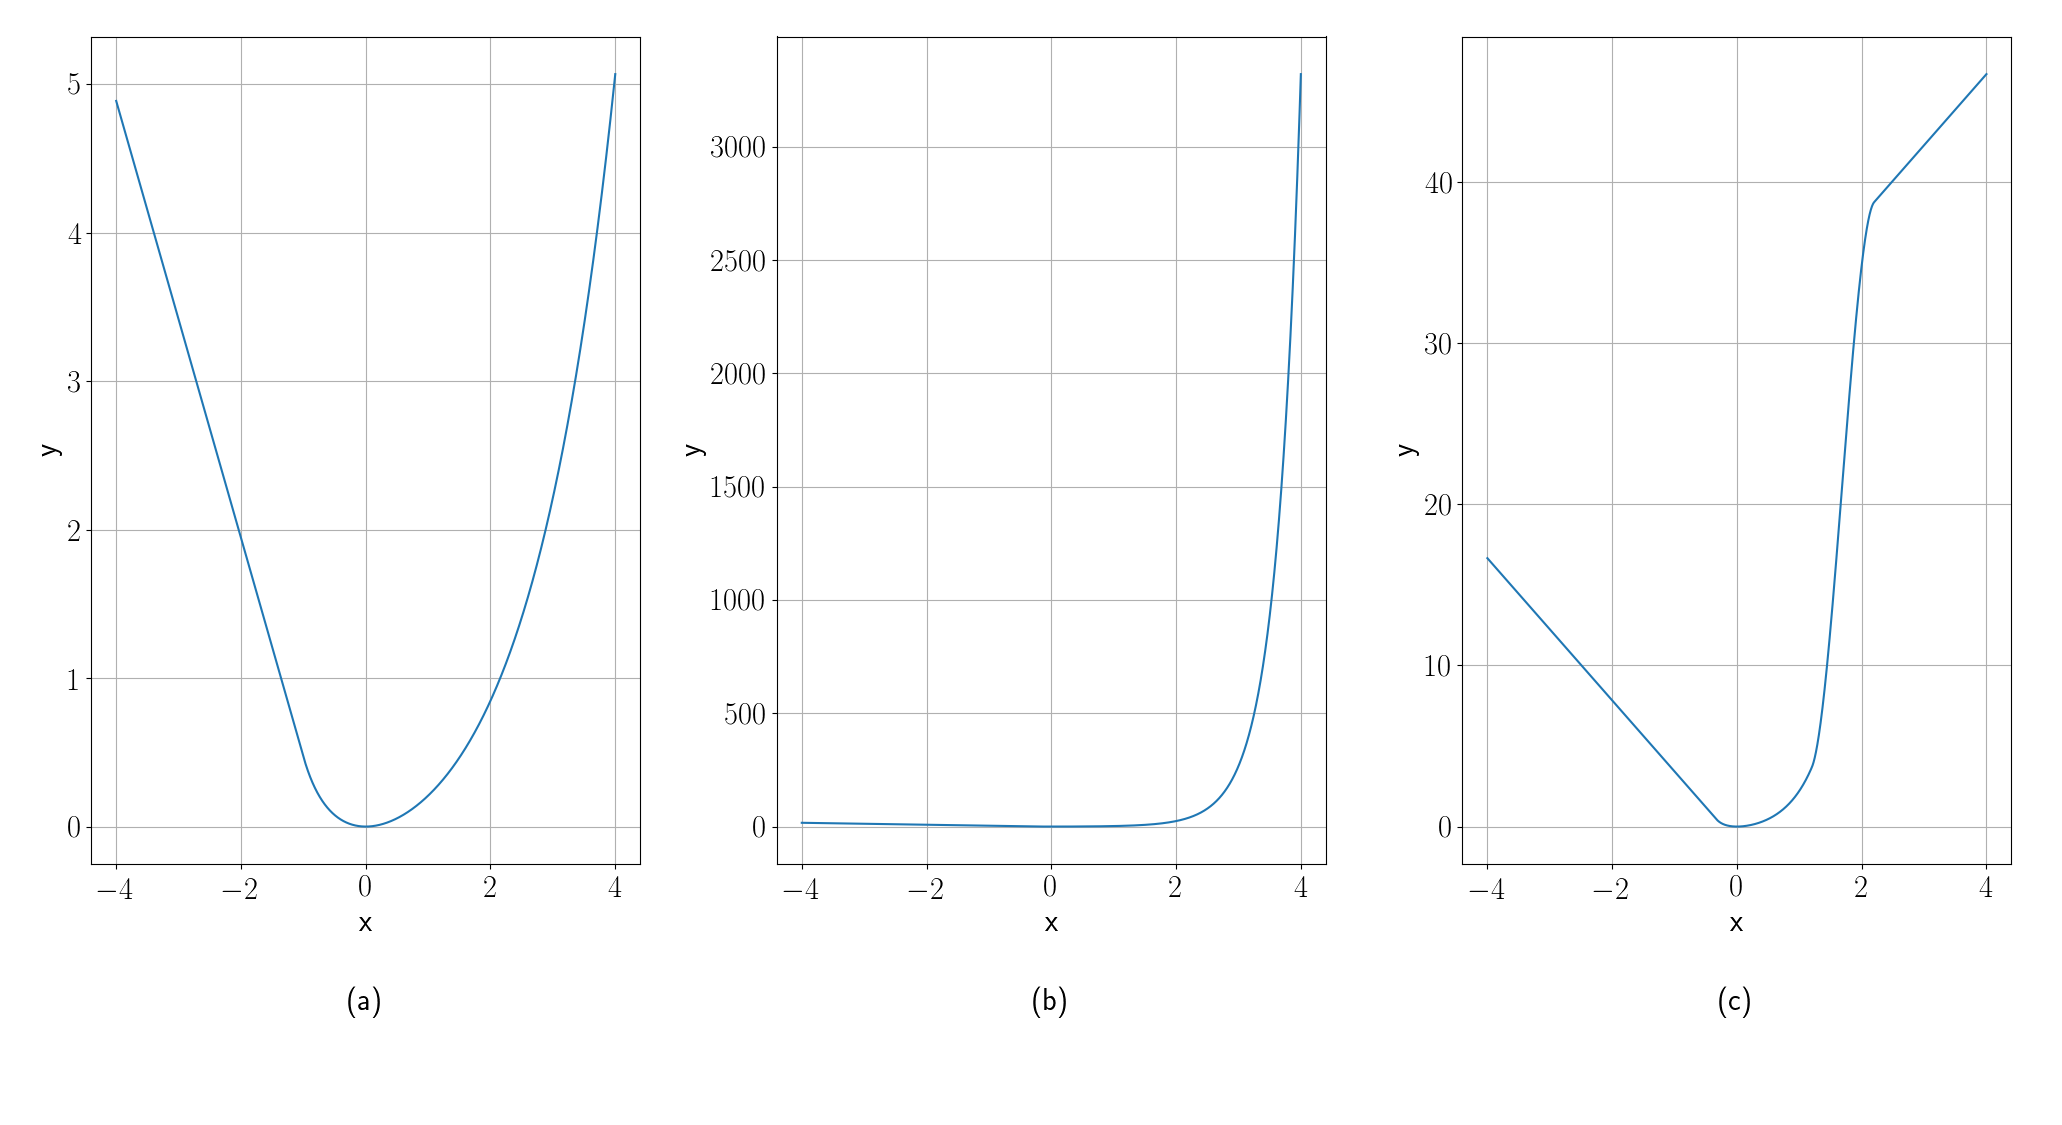
\includegraphics[width=\textwidth]{loss_evolution.png}
\caption[Loss iterations]{Three different stages of the custom loss function. (a): The loss as defined in \eqref{def:loss_original}. For $\left|x\right|<2$ the eyponential part is actually smaller than the linear part. This is not desirable, as for most of our testing the label for pure noise is about $4$ away from the smallest label for a signal. (b): To fix the issue of a too small exponential for some purposes, one can introduce a squish factor, that simply multiplies the input by some fixed value. In this case a squish factor of 3 was used. The values in general are a lot larger. (c): Having a large squish factor as in (b) introduces the problem of too large gradients. For this purpose, a cutoff can be introduced. This cutoff grows linearly with the same slope as the linear part of \eqref{def:loss_squished}. The transition between the exponential and linear part however needs to be of class $C^1$, so that the backpropagation algorithm can optimize. Therefore a spline polynomial connects the two parts.}\label{fig:loss_evolution}
\end{figure}
